\section{Analiza wyników}

\cell
Zaprezentowany w~poprzednim rozdziale model $\textit{GML-Net}$ można by uznać za ukończony, gdyby operował on na obrazach o rozdzielczości $\textit{5000x5000}$. Niestety trenowanie głębokiej sieci neuronowej na obrazach o tak wysokiej rozdzielczości nie jest możliwe ze względu na ograniczoną pojemność kart graficznych, stąd też konieczne było wytrenowanie sieci $\textit{GML-Net}$ na licznych podpróbkach obrazów oryginalnej rozdzielczości. Aby wygenerować finalną predykcję masek dla obrazów o rozdzielczości $\textit{5000x5000}$ postanowiono więc wygenerować predykcje dla ich podpróbek o rozdzielczości $\textit{256x256}$, a następnie te podpróbki miały zostać połączone w jedną łączną maskę o wysokiej rozdzielczości. Taki proces należałoby powtórzyć dla wszystkich zdjęć znajdujących się w zbiorze walidacyjnym po to aby móc dokładnie określić finalną jakość predykcji sieci $\textit{GML-Net}$.

\subsection{Generowanie finalnych predykcji}
Pierwszym etapem generowania finalnych predykcji było wczytanie zapisu najlepszego uzyskanego modelu wraz z odpowiednimi jego hiperparametrami oraz ustawienie go w~trybie ewaluacji.

\cell
\begin{lstlisting}[name=Rozdzial3.1, language=Python]
mdl_from_path = True

if mdl_from_path:
  mdl_n = "ResNet50_wide_UNet_depth_3_BottleNeck_BS_18.pth"
  model_dict = torch.load(mdl_path + mdl_n)
  state_dict = model_dict['model_params']
  trnd_model = GML_Net(layrs_dict=net_ls)
  trnd_model.load_state_dict(state_dict)
  trnd_model.cuda()
  device = torch.device('cuda' if torch.cuda.is_available() else 'cpu')
  trnd_model.eval()
\end{lstlisting}

\cell
\begin{lstlisting}[name=Rozdzial3.1, language=Python]
def g_prms(imgs_arr, img_num):
  mask_path = imgs_arr[img_num, 1]
  image = np.array(Image.open(imgs_arr[img_num, 0]))
  mask = np.array(Image.open(mask_path))
  wind_h = sample_res
  wind_w = sample_res
  img_shp = image.shape
  nm_cls = img_shp[-1] if len(img_shp) > 2 else 1
  img_h = img_shp[0]
  img_w = img_shp[1]
  S_y = sample_res // 2
  S_x = sample_res // 2
  return image, mask, wind_h, wind_w, nm_cls, img_h, img_w, S_y, S_x
\end{lstlisting}


\cell
Przy pomocy funkcji $\textit{g$\_$prms}$ ustalono najważniejsze parametry podziału zdjęć pochodzących ze zbioru walidacyjnego na podpróbki o rozdzielczości $\textit{256x256}$. Postanowiono, iż każde zdjęcie zostanie podzielone na 1444 nakładające się podpróbki, szerokość nakładania się ustalono na połowę wymiaru podpróbki.

\cell
\begin{lstlisting}[name=Rozdzial3.1, language=Python]
def get_wnds(img, msk, wnd_h, wnd_w, nm_cls, img_h, img_w, Sy, Sx):
  G_x = 1 + (img_w - wnd_w) // Sx
  G_y = 1 + (img_h - wnd_h) // Sy
  s_l = Sy * img_w * nm_cls
  s_k = Sx * nm_cls
  s_b = img_w * nm_cls
  s_a = 1 * nm_cls
  img_windows = as_strided(img, shape=(G_y, G_x, wnd_h, wnd_w, nm_cls), 
                          strides=(s_l, s_k, s_b, s_a, 1))
  return img_windows.reshape((G_y * G_x, wnd_h, wnd_w, nm_cls)), G_x, G_y
\end{lstlisting}


\cell
Przy pomocy funkcji $\textit{as$\_$strided}$ pochodzącej z biblioteki $\textit{numpy.lib.stride$\_$tricks}$ przeprowadzono podział każdego ze zdjęć walidacyjnych.

\cell
\begin{lstlisting}[name=Rozdzial3.1, language=Python]
imgs_arr = pd.read_csv("m_inf_v.csv", header=None).values
img_n = 1
img, msk, wnd_h, wnd_w, nm_cls, img_h, img_w, Sy, Sx = g_prms(imgs_arr, 
                                                              img_n)
wnd_img, Gx, Gy = get_wnds(img, msk, wnd_h, wnd_w, nm_cls, img_h, img_w, 
                           Sy, Sx)
fig, axs = plt.subplots(Gx, Gy)
plt.subplots_adjust(wspace=0.1, hspace=0.1)
fig.set_size_inches(20, 20)

for i, ax in enumerate(axs.flat):  
  ax.imshow(wnd_img[i])
  ax.axis('off')
plt.savefig('Podprobki.png', dpi=300, bbox_inches='tight')
\end{lstlisting}

Aby mieć pewność, że podział został przeprowadzony prawidłowo postanowiono zilustrować go przy pomocy mozaiki składającej się z wszystkich podpróbek wybranego zdjęcia (patrz rysunek \ref{fig:podprob1}).

\begin{figure}[!h]
    \centering \includegraphics[width=1.0\linewidth]{Podprobki.png}
    \captionsetup{format=hang}
    \caption{Wybrane zdjęcie pochodzące ze zbioru walidacyjnego rozbite na 1444 podpóbki}
    \label{fig:podprob1}
\end{figure}

\cell
Mając do dyspozycji wszystkie 1444 podpróbki zdjęcia bazowego można było przystąpić do generowania predykcji masek dla każdej z tych podpróbek.
\vspace{1.5cm}

\cell
\begin{lstlisting}[name=Rozdzial3.1, language=Python]
def get_all_preds(reshp_img):
  fin_trans = transforms.Compose([transforms.ToTensor(), 
                                  transforms.Normalize(mean_rgbs, std_rgbs)])
  fin_preds = np.zeros((reshp_img.shape[0], sample_res, sample_res))

  for i in range(0, reshp_img.shape[0], batch_s):
    if i + batch_s > reshp_img.shape[0]:
      continue
    input = reshp_img[i:(i + batch_s), ...]
    trans_input = torch.zeros((input.shape[0], input.shape[3], input.shape[1], 
                              input.shape[2]))
    for j in range(input.shape[0]):
      trans_input[j, ...] = fin_trans(input[j, ...])
    with torch.no_grad():
      pred_base = trnd_model(trans_input.to(device))

    pred_sigm = torch.sigmoid(pred_base).data.cpu().numpy()
    fin_preds[i:(i + batch_s), ...] = pred_sigm
    
  return fin_preds
\end{lstlisting}


\cell
Aby móc efektywnie połączyć uzyskane predykcje w jedną łączną maskę o rozdzielczości $\textit{5000x5000}$ postanowiono skorzystać z dwuwymiarowych okien Hanna zdefiniowanych szerzej w artykule Nicolasa Pielawskiego oraz Caroliny Wählby \textit{Introducing Hann windows for reducing edge-effects in patch-based image segmentation} \cite{pielawski}.

\cell
\begin{lstlisting}[name=Rozdzial3.1, language=Python]
hann_wnd_b = np.zeros((sample_res, sample_res), dtype=float)
hann_wnd_up = np.zeros((sample_res, sample_res), dtype=float)
hann_wnd_down = np.zeros((sample_res, sample_res), dtype=float)
hann_wnd_left = np.zeros((sample_res, sample_res), dtype=float)
hann_wnd_right = np.zeros((sample_res, sample_res), dtype=float)
hann_wnd_up_l = np.zeros((sample_res, sample_res), dtype=float)
hann_wnd_down_l = np.zeros((sample_res, sample_res), dtype=float)
hann_wnd_up_r = np.zeros((sample_res, sample_res), dtype=float)
hann_wnd_down_r = np.zeros((sample_res, sample_res), dtype=float)
\end{lstlisting}


\cell
Autorzy tego artykułu zaproponowali algorytm łączenia podpróbek zdjęć w jedno łączne zdjęcie w czasie realizowania zadań z zakresu semantycznej segmentacji. Ich pomysł opierał się na przemnażaniu predykcji uzyskanych dla poszczególnych podpróbek przez dwuwymiarowe okna Hanna, stanowiące $\textit{de facto}$ macierz wag, która główny nacisk kładzie na predykcje znajdujące się w środku podpróbki - w ten sposób redukowany jest efekt złych predykcji krawędzi.

\cell
\begin{lstlisting}[name=Rozdzial3.1, language=Python]
def hann_up_down_left_right(i, j, h_part, v_part):
  if j < sample_res / 2:
    hann_wnd_up[j, i] = 0.5 * h_part
  else:
    hann_wnd_up[j, i] = 0.25 * h_part * v_part
  
  if j > sample_res / 2:
    hann_wnd_down[j, i] = 0.5 * h_part
  else:
    hann_wnd_down[j, i] = 0.25 * h_part * v_part

  if i < sample_res / 2:
    hann_wnd_left[j, i] = 0.5 * v_part
  else:
    hann_wnd_left[j, i] = 0.25 * h_part * v_part
  
  if i > sample_res / 2:
    hann_wnd_right[j, i] = 0.5 * v_part
  else:
    hann_wnd_right[j, i] = 0.25 * h_part * v_part
\end{lstlisting}


\cell
Nicolas Pielawski i Caroline Wählby zaproponowali również modyfikacje bazowego dwuwymiarowego okna Hanna, dla przypadków gdy predykcja pochodzi z podpróbki znajdującej się na krawędzi zdjęcia bazowego, tak żeby w takich przypadkach położyć nacisk na predykcje znajdujące się na krawędziach podpróbki.

\cell
\begin{lstlisting}[name=Rozdzial3.1, language=Python]
def hann_up_l_up_r(i, j, h_part, v_part):
  if i <= sample_res / 2 and j <= sample_res / 2:
    hann_wnd_up_l[j, i] = 1
  elif i > sample_res / 2 and j < sample_res / 2:
    hann_wnd_up_l[j, i] = 0.5 * h_part
  elif i < sample_res / 2 and j > sample_res / 2:
    hann_wnd_up_l[j, i] = 0.5 * v_part
  else:
    hann_wnd_up_l[j, i] = 0.25 * h_part * v_part

  if i >= sample_res / 2 and j <= sample_res / 2:
    hann_wnd_up_r[j, i] = 1
  elif i < sample_res / 2 and j < sample_res / 2:
    hann_wnd_up_r[j, i] = 0.5 * h_part
  elif i > sample_res / 2 and j > sample_res / 2:
    hann_wnd_up_r[j, i] = 0.5 * v_part
  else:
    hann_wnd_up_r[j, i] = 0.25 * h_part * v_part
\end{lstlisting}


\cell
W ten sposób uzyskano 9 wariantów dwuwymiarowego okna Hanna, których zastosowanie zależało od tego gdzie dana podpróbka znajduje się na obrazie bazowym. Funkcje $\textit{hann$\_$up$\_$down$\_$eft$\_$right}$, $\textit{hann$\_$up$\_$l$\_$up$\_$r}$ oraz $\textit{hann$\_$down$\_$r$\_$down$\_$l}$ zawierają implementacje poszczególnych dwuwymiarowych okien Hanna.

\cell
\begin{lstlisting}[name=Rozdzial3.1, language=Python]
def hann_down_r_down_l(i, j, h_part, v_part):
  if i >= sample_res / 2 and j >= sample_res / 2:
    hann_wnd_down_r[j, i] = 1
  elif i < sample_res / 2 and j > sample_res / 2:
    hann_wnd_down_r[j, i] = 0.5 * h_part
  elif i > sample_res / 2 and j < sample_res / 2:
    hann_wnd_down_r[j, i] = 0.5 * v_part
  else:
    hann_wnd_down_r[j, i] = 0.25 * h_part * v_part
  if i <= sample_res / 2 and j >= sample_res / 2:
    hann_wnd_down_l[j, i] = 1
  elif i > sample_res / 2 and j > sample_res / 2:
    hann_wnd_down_l[j, i] = 0.5 * h_part
  elif i < sample_res / 2 and j < sample_res / 2:
    hann_wnd_down_l[j, i] = 0.5 * v_part
  else:
    hann_wnd_down_l[j, i] = 0.25 * h_part * v_part
\end{lstlisting}


\cell
Rysunek \ref{fig:hann1} prezentuje wizualizację wszystkich dziewięciu okien Hanna, które w dalszej części niniejszego podrozdziału posłużą do połączenia predykcji uzyskanych z podpróbek w jedną łączną maskę predykcji.
\vspace{1cm}

\cell
\begin{lstlisting}[name=Rozdzial3.1, language=Python]
for i in range(sample_res):
  for j in range(sample_res):
    h_part = (1 - np.cos((2 * np.pi * i) / (sample_res - 1)))
    v_part = (1 - np.cos((2 * np.pi * j) / (sample_res - 1)))
    hann_wnd_b[j, i] = 0.25 * h_part * v_part
    hann_up_down_left_right(i, j, h_part, v_part)
    hann_up_l_up_r(i, j, h_part, v_part)
    hann_down_r_down_l(i, j, h_part, v_part)
\end{lstlisting}

\begin{figure}[!h]
    \centering 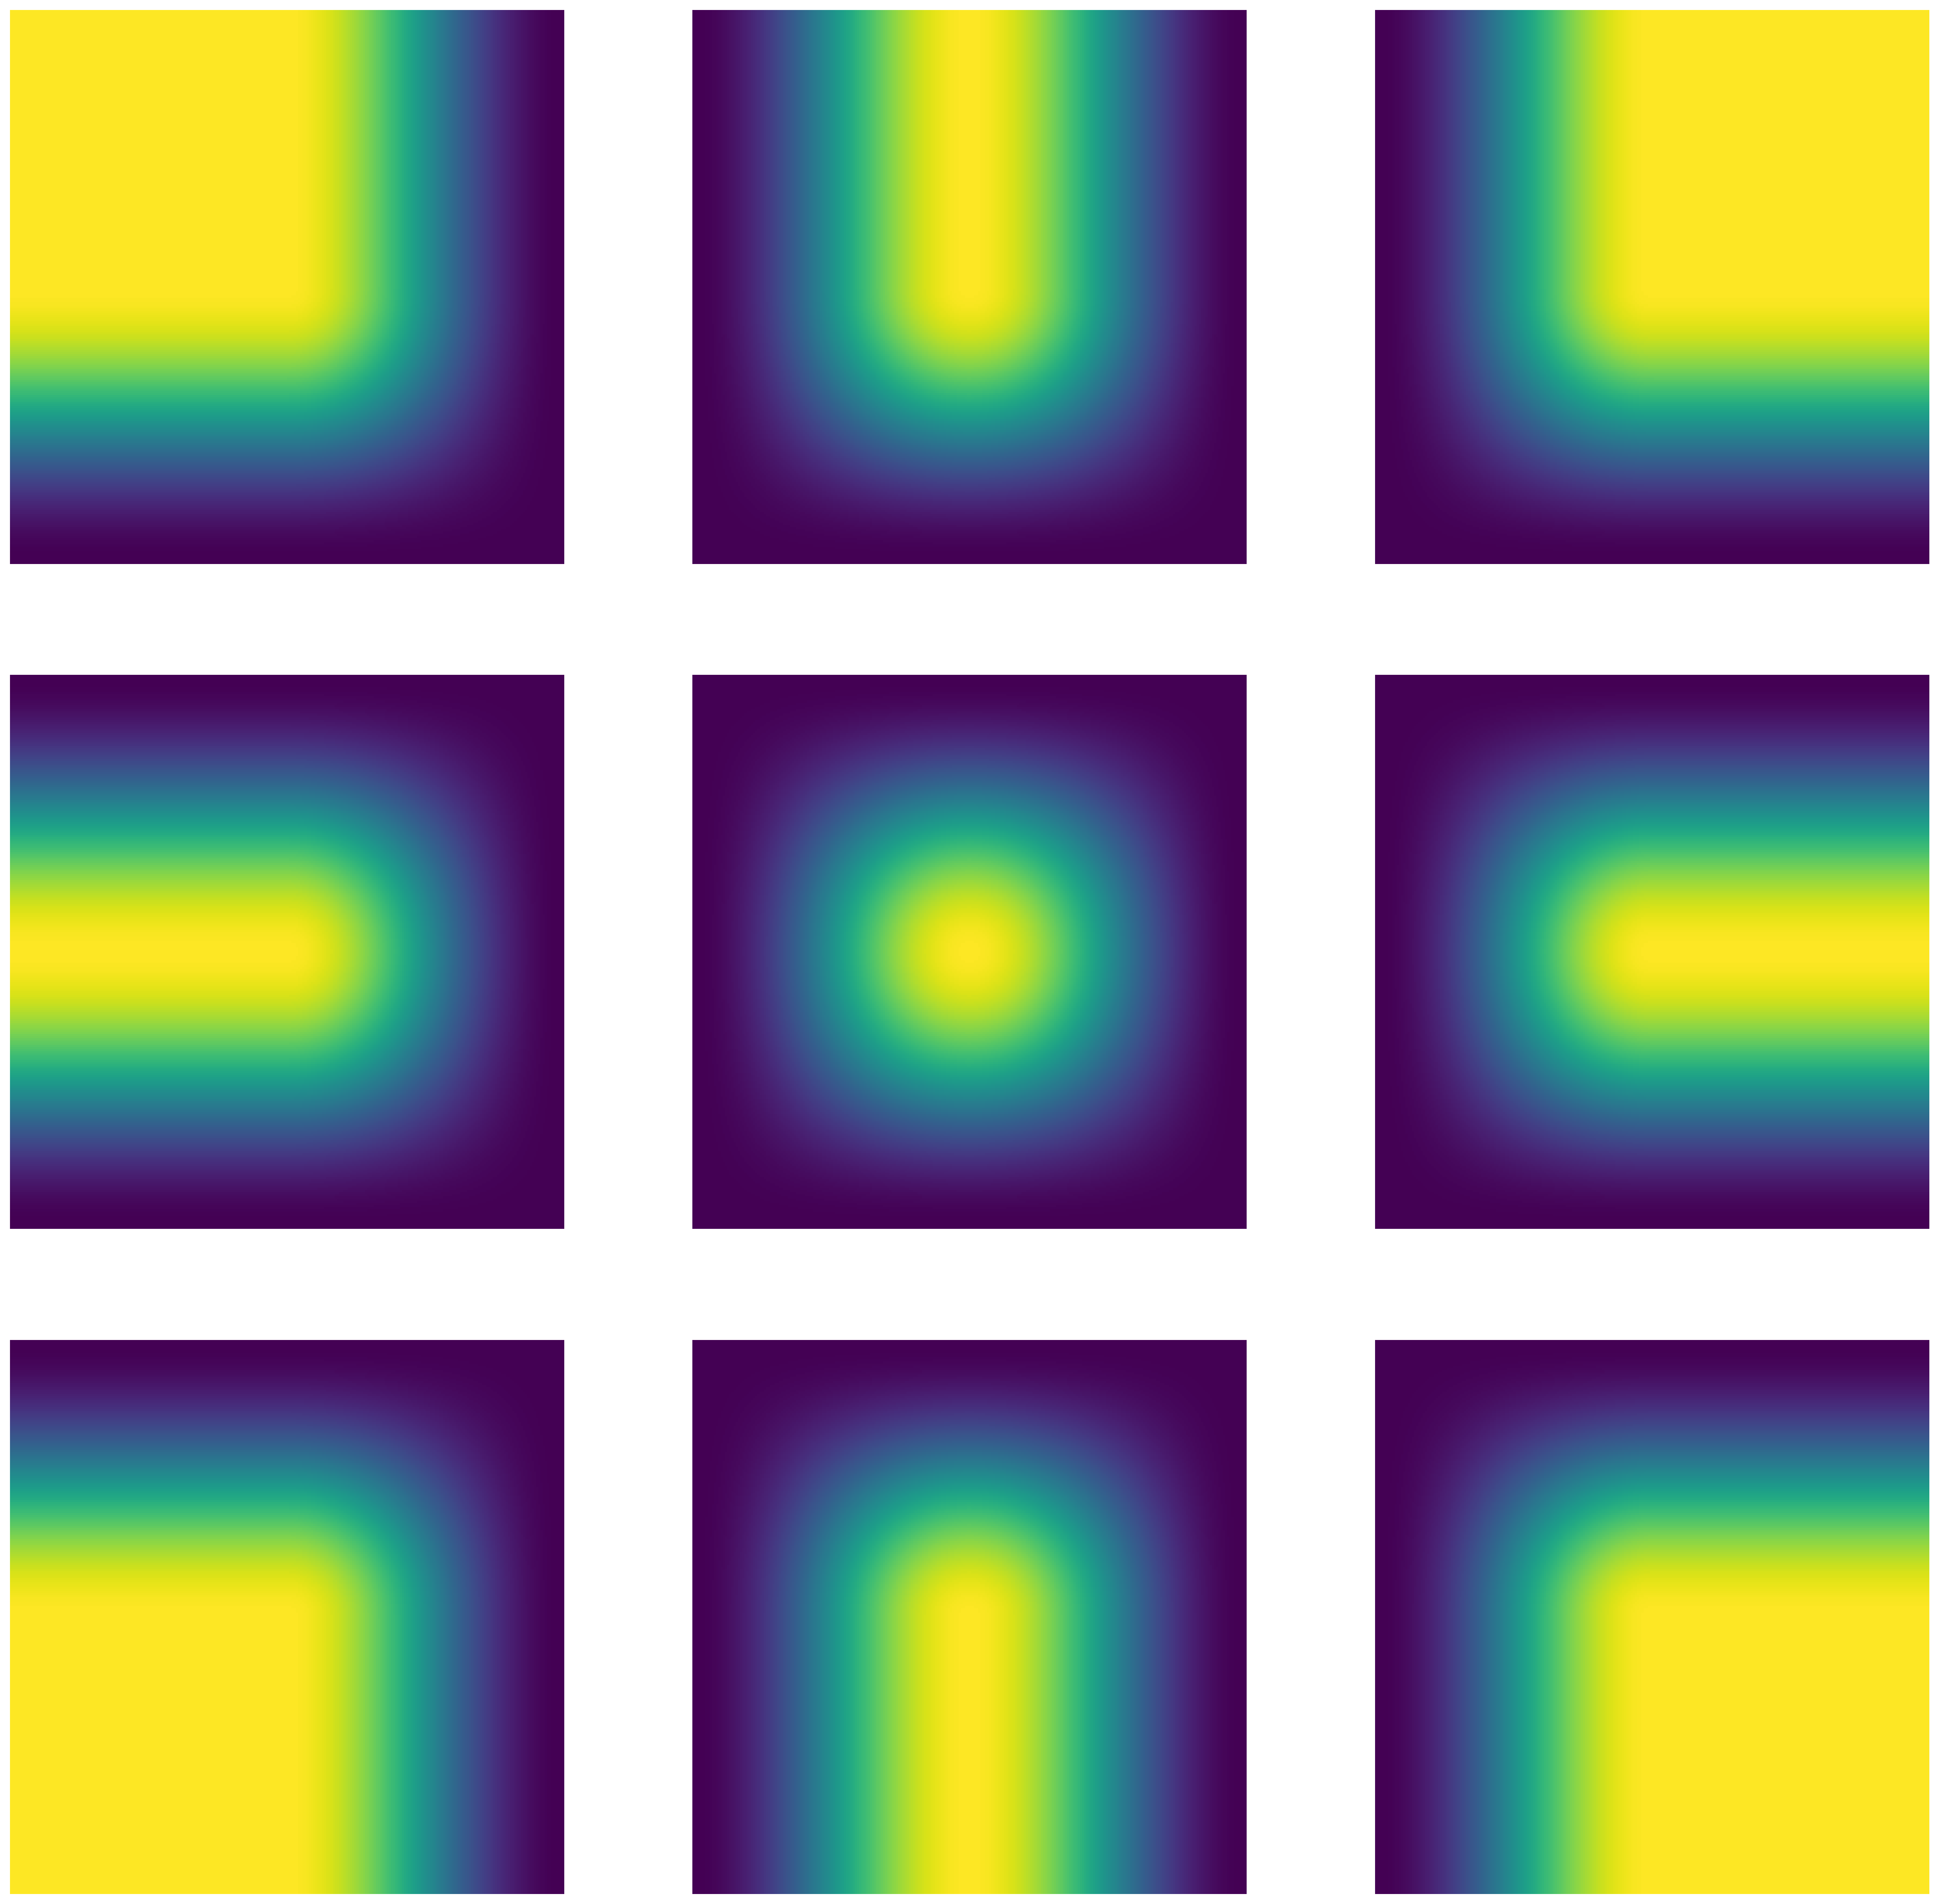
\includegraphics[width=1.0\linewidth]{Okna Hanna.png}
    \captionsetup{format=hang}
    \caption{Wizualizacja dziewięciu okien Hanna 2D służących do właściwego ważenia predykcji poszczególnych fragmentów zdjęcia bazowego}
    \label{fig:hann1}
\end{figure}
\vspace{1cm}

\cell
\begin{lstlisting}[name=Rozdzial3.1, language=Python]
f2, axarr2 = plt.subplots(nrows=3, ncols=3, figsize=(25, 25))
axarr2[0, 0].imshow(hann_wnd_up_l, cmap='viridis')
axarr2[1, 0].imshow(hann_wnd_left, cmap='viridis')
axarr2[2, 0].imshow(hann_wnd_down_l, cmap='viridis')
axarr2[0, 1].imshow(hann_wnd_up, cmap='viridis')
axarr2[1, 1].imshow(hann_wnd_b, cmap='viridis')
axarr2[2, 1].imshow(hann_wnd_down, cmap='viridis')
axarr2[0, 2].imshow(hann_wnd_up_r, cmap='viridis')
axarr2[1, 2].imshow(hann_wnd_right, cmap='viridis')
axarr2[2, 2].imshow(hann_wnd_down_r, cmap='viridis')
axarr2[0, 0].axis('off')
axarr2[1, 0].axis('off')
axarr2[2, 0].axis('off')
axarr2[0, 1].axis('off')
axarr2[1, 1].axis('off')
axarr2[2, 1].axis('off')
axarr2[0, 2].axis('off')
axarr2[1, 2].axis('off')
axarr2[2, 2].axis('off')
plt.savefig('Okna Hanna.png', dpi=300, bbox_inches='tight')
\end{lstlisting}

\cell
Funkcja $\textit{choose$\_$proper$\_$hann}$ służy do wyboru odpowiedniego dwuwymiarowego okna Hanna, w zależności od tego, z której części bazowego zdjęcia walidacyjnego dana podpróbka została pobrana.

\cell
\begin{lstlisting}[name=Rozdzial3.1, language=Python]
def choose_proper_hann(i, j, max_shp):
  if j == 0 and i == 0:
    curr_hann = hann_wnd_up_l
  elif i == 0 and j != 0 and j != max_shp - 1:
    curr_hann = hann_wnd_up
  elif i == 0 and j == max_shp - 1:
    curr_hann = hann_wnd_up_r
  elif j == 0 and i != 0 and i != max_shp - 1:
    curr_hann = hann_wnd_left
  elif j == 0 and i == max_shp - 1:
    curr_hann = hann_wnd_down_l
  elif j == max_shp - 1 and i != 0 and i != max_shp - 1:
    curr_hann = hann_wnd_right
  elif j == max_shp - 1 and i == max_shp - 1:
    curr_hann = hann_wnd_down_r
  elif j != 0 and j != max_shp - 1  and i == max_shp - 1:
    curr_hann = hann_wnd_down
  else:
    curr_hann = hann_wnd_b
  return curr_hann
\end{lstlisting}


\cell
Przy pomocy funkcji $\textit{get$\_$fin$\_$mask}$ realizowane jest generowanie finalnej maski dla poszczególnych zdjęć ze zbioru walidacyjnego. Funkcja ta przechodzi przez predykcje wygenerowane dla wszystkich podpróbek, przemnaża je przez odpowiednie okna Hanna i~nanosi we właściwym miejscu finalnej maski $\textit{5000x5000}$. 

\cell
\begin{lstlisting}[name=Rozdzial3.1, language=Python]
def get_fin_mask(fin_preds, Gy, Gx, wnd_h, wnd_w, img_h, img_w, Sy, Sx):
  rshp_fin_preds = fin_preds.reshape((Gy, Gx, wnd_h, wnd_w))
  fin_image_mask = np.zeros((img_h, img_w))
  end_x = sample_res
  strt_x = 0
  for i in range(Gy):
    end_y = sample_res
    strt_y = 0
    for j in range(Gx):
      curr_p = rshp_fin_preds[i, j]
      curr_h = choose_proper_hann(i, j, Gy)
      fin_image_mask[strt_x:end_x, strt_y:end_y] += np.multiply(curr_p, curr_h)
      strt_y += Sy
      end_y += Sy
    strt_x += Sx
    end_x += Sx
  return fin_image_mask
\end{lstlisting}

\subsection{Pomiar efektywności sieci \emph{GML-Net}}

\cell
Poniższe obrazy wizualizują skuteczność sieci $\textit{GML-Net}$ w detekcji budynków na zdjęciach lotniczych na przykładzie losowo wybranego zdjęcia ze zbioru walidacyjnego.

\cell
\begin{lstlisting}[name=Rozdzial3.1, language=Python]
imgs_arr = pd.read_csv("m_inf_v.csv", header=None).values
img_n = 1
final_f1s = []
final_iou = []
final_acc = []
final_ssim = []
pred_time = []
img_time = []
img, msk, wnd_h, wnd_w, nm_cls, img_h, img_w, Sy, Sx = g_prms(imgs_arr, img_n)
wnd_img, Gx, Gy = get_wnds(img, msk, wnd_h, wnd_w, nm_cls, img_h, img_w, Sy, Sx)
fin_preds = get_all_preds(wnd_img)
f_img_msk = get_fin_mask(fin_preds, Gy, Gx, wnd_h, wnd_w, img_h, img_w, Sy, Sx)
\end{lstlisting}

\begin{figure}[!h]
    \centering \includegraphics[width=1.0\linewidth]{Maska GT.png}
    \captionsetup{format=hang}
    \caption{Oryginalna maska (\textit{ground truth})}
    \label{fig:predGT1}
\end{figure}

\cell
Porównanie wizualne rysunku \ref{fig:predGT1} z rysunkiem \ref{fig:predGT2} wskazuje, iż różnice w predykcji maski przez sieć $\textit{GML-Net}$ a faktyczną maską $\textit{ground truth}$ nie są istotne.

\begin{figure}[!h]
    \centering \includegraphics[width=1.0\linewidth]{Predykcja sieci.png}
    \captionsetup{format=hang}
    \caption{Maska wygenerowana przez sieć \textit{GML-Net}}
    \label{fig:predGT2}
\end{figure}

\cell
\begin{lstlisting}[name=Rozdzial3.1, language=Python]
img_rgba = np.ones((img.shape[0], img.shape[1], 4), dtype=np.uint8) * 255
img_rgba[..., :3] = img
mask_rgba = np.zeros((img.shape[0], img.shape[1], 4), dtype=np.uint8)
mask_rgba[msk == 255, ...] = [0, 0, 255, 180]
pred_mask_rgba = np.zeros((img.shape[0], img.shape[1], 4), dtype=np.uint8)
pred_mask_rgba[f_img_msk > loss_thres, ...] = [128, 0, 128, 180]

f2, axarr2 = plt.subplots(nrows=1, ncols=2, figsize=(25, 25))
axarr2[0].set_title("Maska ground truth\n", color='black', fontweight="bold",
                    fontsize=25)
axarr2[0].imshow(img_rgba)
axarr2[0].imshow(mask_rgba, alpha=0.6)
axarr2[0].axis('off')
axarr2[1].imshow(img_rgba)
axarr2[1].imshow(pred_mask_rgba, alpha=0.6)
axarr2[1].axis('off')
axarr2[1].set_title("Maska uzyskana z sieci GML-Net\n", color='black', 
                    fontweight="bold", fontsize=25)
                    
plt.savefig('Predykacja vs. maska.png', dpi=300, bbox_inches='tight')
\end{lstlisting}

\cell
\begin{lstlisting}[name=Rozdzial3.1, language=Python]
def calc_metrics(f_img_msk, msk):
  prd2 = f_img_msk > loss_thres
  trgt2 = msk == 255
  intrs = (prd2 * trgt2).sum()
  
  f1s = torch.True_divide(2. * intrs, prd2.sum() + trgt2.sum())
  f1s = f1s.cpu().numpy().item(0)
  union = (prd2 + trgt2).sum()
  
  iou = torch.True_divide(intrs, union).cpu().numpy().item(0)
  acc = torch.True_divide(intrs + (~prd2 * ~trgt2).sum(), prd2.size)
  acc = acc.cpu().numpy().item(0)
  
  prd3 = torch.tensor(np.expand_dims(prd2, axis=0)).cuda()
  trgt3 = torch.tensor(np.expand_dims(trgt2, axis=0)).cuda()
  ssim = ssim_index(prd3, trgt3).cpu().numpy().item(0)
  
  return f1s, iou, acc, ssim

f1s, iou, acc, ssim = calc_metrics(f_img_msk, msk)
\end{lstlisting}


\cell
Wartości poszczególnych metryk wyliczone dla powyższego losowego zdjęcia pochodzącego ze zbioru walidacyjnego potwierdzają obserwacje wizualne wskazujące na dobrą jakość predykcji. Wartości tych metryk są następujące: $\textit{OA}$ = 97,66$\%$, $\textit{IoU}$ = 80,10$\%$, $\textit{F1S}$ = 88,95$\%$ oraz $\textit{SSIM}$ = 96,26$\%$.
\vspace{1cm}

\cell
\begin{lstlisting}[name=Rozdzial3.1, language=Python]
for i in range(len(imgs_arr)):
  since0 = time.time()
  img, msk, wnd_h, wnd_w, nm_cls, img_h, img_w, Sy, Sx = g_prms(imgs_arr, i)
  wnd_i, Gx, Gy = get_wnds(img, msk, wnd_h, wnd_w, nm_cls, img_h, img_w, 
                           Sy, Sx)
  fin_p = get_all_preds(wnd_i)
  since1 = time.time()
  f_img_msk = get_fin_mask(fin_p, Gy, Gx, wnd_h, wnd_w, img_h, img_w,
                           Sy, Sx)
  pred_time += [time.time() - since1]
  img_time += [time.time() - since0]
  f1s, iou, acc, ssim = calc_metrics(f_img_msk, msk)                                                        
  final_f1s += [f1s]
  final_iou += [iou]
  final_acc += [acc]
  final_ssim += [ssim]

joined_time = sum(img_time)
av_img_time = sum(img_time) / len(imgs_arr)
avg_pred_time = sum(pred_time) / (len(imgs_arr) * Gx * Gy)
\end{lstlisting}

\cell
Sieć $\textit{GML-Net}$ osiągnęła zadowalającą finalną skuteczność na zbiorze walidacyjnym przy predykcji masek o rozmiarach $\textit{5000x5000}$ - uzyskano następujące finalne wartości metryk: \textit{OA} = 96,44\%, \textit{IoU} = 75,97\%, \textit{F1S} = 86,07\% oraz \textit{SSIM} = 94,55\%. Wyniki te zostały uzyskane przy średnim czasie generowania predykcji jednej maski \emph{256x256} na poziomie 0,0003 sekundy oraz średnim czasie generowania predykcji maski łącznego obrazka \emph{5000x5000} na poziomie 15 sekund.
\vspace{0.5cm}

\begin{table}[!h]
\centering
\begin{tabular}{|M{3cm}|M{5.5cm}|M{5.5cm}|}
\hline
\rowcolor{gray!50}
\textbf{Rodzaj metryki} & \textbf{Wyniki dla masek 256x256} & \textbf{Wyniki dla masek 5000x5000} \\ 
 \hline 
\textbf{OA} & 97,08\% & 96,44\% \\
 \hline 
\textbf{IoU} & 82,42\% & 75,97\% \\
 \hline 
\textbf{F1S} & 88,22\% & 86,07\% \\
 \hline 
\textbf{SSIM} & 95,46\% & 94,55\% \\
 \hline 
\end{tabular}
\caption{Podsumowanie różnic pomiędzy metrykami jakości predykcji sieci \textit{GML-Net} dla masek \emph{256x256} a~tymi samymi metrykami dla masek \emph{5000x5000}.}
\label{tab:tabela2}
\end{table}

Jak można się było spodziewać metryki jakości predykcji modelu wyliczane na poziomie pełnych zdjęć o wysokiej rozdzielczości są gorsze od metryk wyliczanych na poziomie podpróbek o rozdzielczości $\textit{256x256}$. Ogólna dokładność pogarsza się o 0,64 punktu procentowego, współczynnik podobieństwa Jaccarda spada aż o 6,45 p.p., wynik $\textit{F1}$ jest niższy o 2,35 p.p. a indeks podobieństwa strukturalnego jest gorszy o 0,91 p.p. 

\subsection{Uzyskane wyniki na tle literatury badawczej}

Tabela \ref{tab:tabela3} przywołuje ponownie wyniki uzyskane na zbiorze \textit{Inria Aerial Image Labeling Dataset} przez autorów, których prace zostały omówione w~przeglądzie literatury. Uzyskane przez nich wyniki dotyczą zbioru testowego \emph{IAILD}, natomiast opisywane, jak dotąd, wartości metryk jakości predykcji sieci \textit{GML-Net} dotyczyły wyłącznie zbioru walidacyjnego. Aby więc móc porównywać skuteczność modelu opisywanego w~bieżącej pracy na tle skuteczności innych modeli, należałoby policzyć odpowiednie metryki jakości predykcji sieci \textit{GML-Net} na zbiorze testowym.

\vspace{0.5cm}
\begin{table}[!h]
\centering
\begin{tabular}{|M{7cm}|M{4cm}|}
\hline
\rowcolor{gray!50}
\textbf{Tytuł artykułu} & \textbf{Uzyskane wyniki} \\ \hline &\\[0.1cm]

\emph{Multi-Task Learning for Segmentation of Building Footprints with Deep Neural Networks} \cite{bischke} & \makecell{OA: 95.17\% \\ IoU: 70.14\%} \\[0.1cm] &\\ \hline &\\[0.1cm]

\emph{Semantic Segmentation from Remote Sensor Data and the Exploitation of Latent Learning for Classification of Auxiliary Tasks} \cite{chatterjee} & \makecell{OA: 97.14\% \\ IoU: 80.32\%} \\[0.1cm] &\\ \hline &\\[0.1cm]

\emph{Building Footprint Generation by Integrating Convolution Neural Network with Feature Pairwise Conditional Random Field (FPCRF)} \cite{zhu} & \makecell{OA: 95.81\% \\ F1S: 87.65\% \\ IoU: 74.79\%} \\[0.1cm] &\\ \hline &\\[0.1cm]

\emph{Polygonal Building Segmentation by Frame Field Learning} \cite{girard} & \makecell{IoU: 78.00\%} \\[0.1cm] &\\ \hline
\end{tabular}
\caption{Podsumowanie wyników uzyskanych na zbiorze \textit{Inria Aerial Image Labeling Dataset} przez autorów innych badań zajmujących się problematyką detekcji budynków na zdjęciach lotniczych.}
\label{tab:tabela3}
\end{table}

Niestety nie można zrobić tego samodzielnie, gdyż autorzy zbioru \textit{Inria Aerial Image Labeling Dataset} nie udostępnili masek 
\emph{ground truth} dla zbioru testowego. Przygotowali oni jednak formularz na stronie internetowej \emph{IAILD} (\url{https://www.lri.fr/~gcharpia/aerial_benchmark}), w~ramach którego możliwe jest przesłanie, do autorów wykorzystywanego w~bieżącej pracy zbioru danych, predykcji 180~masek dla zbioru testowego. Po wysłaniu takich danych, po pewnym czasie, autorzy \textit{Inria Aerial Image Labeling Dataset} odsyłają, na podany w~formularzu adres \emph{e-mail}, wyliczone przez nich wartości metryk \emph{IoU} oraz \emph{OA}, w~podziale na wyniki dla poszczególnych miast ze zbioru testowego. 

\begin{table}[!h]
\centering
\begin{tabular}{|M{7cm}|M{3cm}|M{3cm}|}
\hline
\rowcolor{gray!50}
\textbf{Miasto} & \textbf{OA} & \textbf{IoU} \\ \hline
Bellingham & 97,11\% & 71,39\% \\ \hline
Bloomington & 97,34\% & 71,83\% \\ \hline
Innsbruck & 96,99\% & 74,89\% \\ \hline
San Francisco & 91,72\% & 74,98\% \\ \hline
Tyrol Wschodni & 98,01\% &  77,85\% \\ \hline
\textbf{Łącznie:} & \textbf{96,23\%} & \textbf{74,42\%} \\ \hline
\end{tabular}
\caption{Podsumowanie wyników sieci \textit{GML-Net} dla zbioru testowego \textit{IAILD}}
\label{tab:tabela4}
\end{table}

Tabela \ref{tab:tabela4} przedstawia wskaźniki jakości predykcji sieci \textit{GML-Net} dla zbioru testowego \textit{IAILD}, wyliczone przez autorów tego zbioru po przesłaniu im 180~predykcji masek. Jak widać omawiana w~bieżącym rozdziale sieć osiągnęła łączną skuteczność mierzoną przy pomocy metryki \textit{OA} na poziomie 96,23\% a~mierzoną przy pomocy metryki \textit{IoU} na poziomie 74,42\%. Najlepsze wyniki sieć \textit{GML-Net} uzyskała dla miasta Tyrol Wschodni, a najgorsze dla miast San Francisco (pod kątem \textit{OA}) oraz Bellingham (pod kątem \textit{IoU}). 

Porównując uzyskane wyniki do wyników zaprezentowanych w~przeglądzie literatury można śmiało stwierdzić, iż sieć \textit{GML-Net} jest w~stanie generować wyniki o~zbliżonej jakości do modeli przedstawionych w~literaturze, odstając o~zaledwie niecały punkt procentowy od najlepszego wyniku pod kątem metryki \textit{OA} i~o~niecałe sześć punktów procentowych pod kątem metryki \textit{IoU}. Wyniki uzyskane przez sieć \textit{GML-Net} można również porównać do wyników prezentowanych przez autorów zbioru  \textit{Inria Aerial Image Labeling Dataset} na ich stronie internetowej (\url{https://project.inria.fr/aerialimagelabeling/leaderboard}). Znajduje się tam tabela przedstawiająca wartości uzyskiwanych metryk \textit{OA} i \textit{IoU} dla 110~modeli, których autorzy zgodzili się na publikację wskaźników jakości predykcji ich sieci. Średnia wartość ogólnej dokładności dla tych 110~modeli wynosi 95,46\%, a~średnia wartość indeksu Jaccarda wynosi 70,02\%, co oznacza, iż sieć \textit{GML-Net} uzyskuje wyniki istotnie wyższe od średnich dla tego zbioru - mówiąc dokładniej, zajmuje 29. miejsce pod kątem \textit{OA} oraz 30 pod kątem \textit{IoU}.